\documentclass[border=7pt]{standalone}
\usepackage{amsmath,amssymb,bm,mathtools}
\usepackage[fontset=none]{ctex}
\setCJKmainfont{Songti SC}\setCJKsansfont{PingFang SC}
\usepackage{tikz}\usetikzlibrary{arrows.meta,calc,patterns,angles,quotes,decorations.markings,decorations.pathmorphing}
\newcommand{\dd}{\mathop{}\!\mathrm d}
\definecolor{blue}{HTML}{235789}\definecolor{red}{HTML}{BC4B41}
\tikzset{axis/.style={->,>=Stealth,line width=.55pt},world/.style={line width=.9pt},flow/.style={->,>=Stealth,line width=.85pt},ray/.style={->,>=Stealth,line width=.85pt},guide/.style={dashed,line width=.4pt},aux/.style={dashed,line width=.4pt},dim/.style={<->,>=Stealth,line width=.5pt},every node/.style={font=\normalsize},force/.style={->,>=Stealth,very thick},gas/.style={fill=blue!7}}
\begin{document}
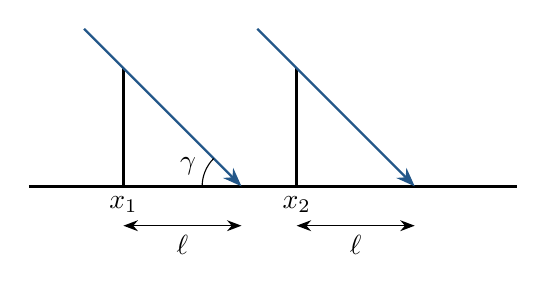
\begin{tikzpicture}
\draw[world](0,0)--(6.2,0);\draw[world](1.2,0)--(1.2,1.5) (3.4,0)--(3.4,1.5);
\draw[ray,blue](.7,2)--(2.7,0);\draw[ray,blue](2.9,2)--(4.9,0);
\draw[dim](1.2,-.5)--(2.7,-.5)node[midway,below]{$\ell$};
\draw[dim](3.4,-.5)--(4.9,-.5)node[midway,below]{$\ell$};
\draw(2.2,0)arc(180:135:.5);\node at(2.02,.25){$\gamma$};
\node[below]at(1.2,0){$x_1$};\node[below]at(3.4,0){$x_2$};
\end{tikzpicture}
\end{document}
